\chapter{Results}
\label{chapter:results}



 

The pressure mat frames are mapped with color scheme Jet and Gaussian interpolation is used to get the final output. Since there was huge difficulties for a proper and careful calibration in the overall pressure mat we could not get highly satisfactory results. But the mat detected areas corresponding to high pressure approximately. More statisfactory image was obtained for feet when standing on the mattress. \begin{figure*}
    \vspace{-0.7cm}
      \centering
      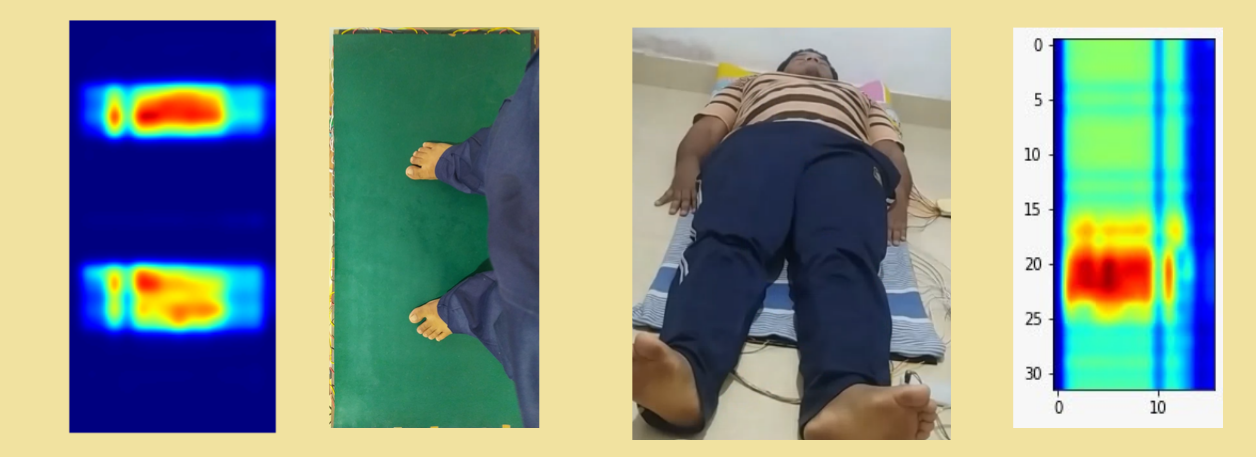
\includegraphics[width=\textwidth]{figs/mat_frames.png}
      \vspace{-0.2cm}
      \caption[Mat frames]{Pressure mat frames}
      \label{fig:mat_frames}
\vspace{1.0cm}
\end{figure*}

Several 1.2kg discs were used to check parts of the mattress.

When an pressure image is sent to the server end point and the posture is detected. Then there are particular ulceration points that are active for that posture. Providing the pressure image and these ulceration point names as the input bounding box parameters can be obtained.
\begin{figure*}[t]
    \vspace{-0.7cm}
      \centering
      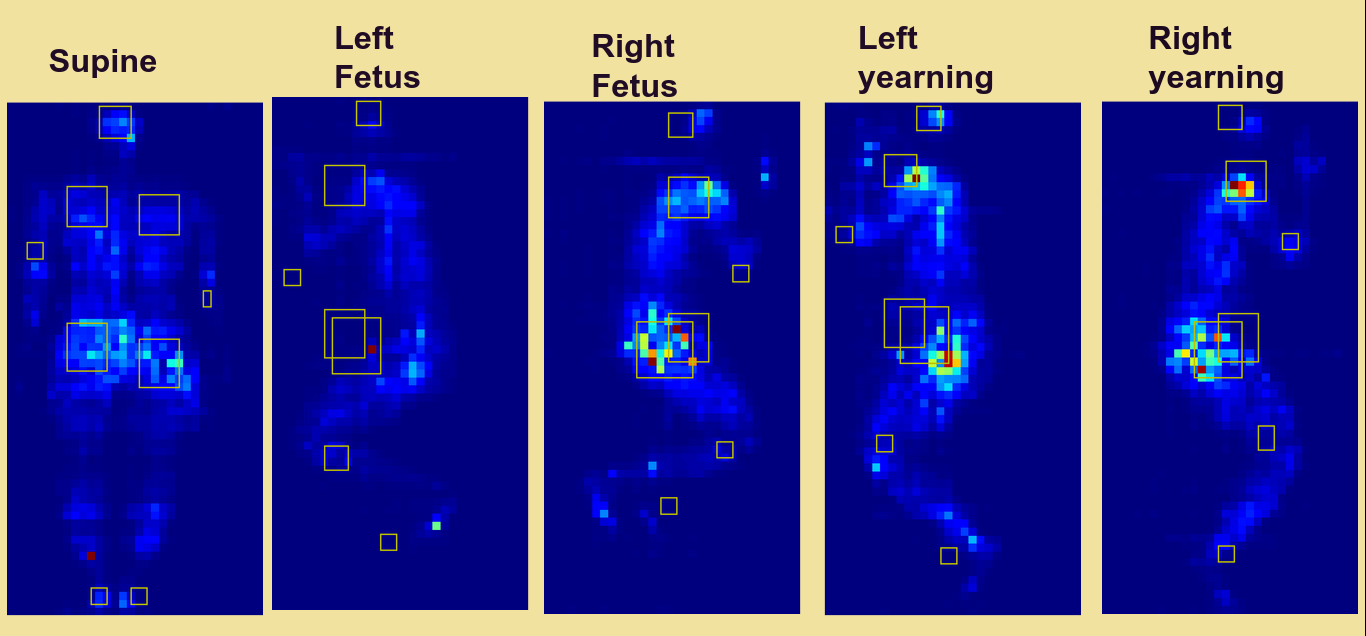
\includegraphics[width=\textwidth]{figs/ml_result.png}
      \vspace{-0.2cm}
      \caption[Results from Neural Network Models]{Results from Neural Network Models}
      \label{fig:mlresult}
\vspace{1.0cm}
\end{figure*}
All five postures classified correctly and bounding boxes are marked appropriately as in the figures.

When ulceration points are located the pressure of these points can be found. We simulated temporal behavour and repositioning using the dataset by University of Dallas.

Repositioning considerably shifts the pressure distribution. 




